% !Mode:: "TeX:UTF-8"
\chapter{绪论}

\section{研究背景}

近些年来,以神经网络(Neural Network)为工具的深度学习(Deep Learning)\upcite{dl}在很多领域都取得了重大的成功,如计算机视觉(Computer Vision),自然语言处理等(Natural Language Process)。随着神经网络模型研究的深入和训练速度的加快,产生了大量的模型。同时,针对不同的使用需求,也产生了大量的异构的硬件设备,如服务器,移动手机,一些专用的加速器等。所以,在多种硬件设备上使用神经网络模型的需求越来越多。传统的使用方式是把神经网络模型部署在服务器上,硬件设备通过网络来调用模型。这样的使用方式无法在离线的情况下使用,同时会占用额外的网络资源。相反,把模型部署在具体的硬件设备上可以降低网络的延迟和负载,同时用户的数据不通过网络进行传输,也可以提高用户的隐私。

但是,把模型部署在硬件设备上面临着很多困难。首先,目前存在着很多的深度学习框架,如Pytorch\upcite{pytorch},Tensorflow\upcite{tensorflow},Caffe\upcite{caffe},MXNet\upcite{mxnet}等,得到的模型结构都有所不同。其次,也存在着很多异构的硬件设备如服务器端CPU,GPU,移动端CPU,GPU,FPGA,TPU\upcite{tpu},在架构上都有所不同。所以,需要一个统一的方式把不同框架的模型部署到异构的硬件设备上。同时,神经网络模型需要占用庞大的计算资源,而一些硬件设备的计算资源往往比较匮乏,所以还需要对部署的模型进行一些优化。

所以,研究人员希望通过编译的技术来解决这个问题,通过编译,对不同框架的模型生成在具体硬件设备上的可执行代码,同时在编译过程中进行一些面向计算图和面向硬件设备的优化。TVM(Open Deep Learning Compiler Stack)\upcite{tvm},一个深度学习的编译器\upcite{dlcompiler}。可以提供端到端的编译流程。

\section{研究目的}

尽管TVM已经提供了较为方便的端到端的编译流程,但是对于TVM的使用仍较为复杂。
主要的难点有以下几个方面:
\begin{enumerate}
    \item {用户需要编译TVM的运行库。}
    \item {用户需要下载很多库,如Cuda(Parallel Computing Platform)\upcite{cuda},LLVM(Compiler)等。}
    \item {用户需要学习TVM部署到服务器,Android,FPGA等硬件设备的流程。需要对TVM的API有一定的了解,同时也需要对系统等方面的知识有一定的了解。}
\end{enumerate}
鉴于以上几个难点,本篇论文基于TVM,把TVM进一步的封装为异构计算的平台,实现一个统一,简洁的接口,使得用户通过该接口能够把不同框架的模型部署到异构的硬件设备上,而不需要处理以上提到的难点,进一步简化部署的流程,降低部署的难度。该平台需要支持Pytorch,Tensorflow,Keras,Onnx,MXNet等深度学习框架,需要能够部署到服务器,安卓设备,树莓派,和FPGA等硬件设备上。


\section{研究意义}

首先,神经网络模型的功能日益丰富,多种硬件设备对神经网络模型的需求日益增多。传统的模型部署到异构设备的流程复杂,且需要很多的人工的调整,浪费了大量的人力。所以,提供一个统一的,易于使用的接口,同时保持与手动调整相近或更优的准确度,能够节省大量的人力。

其次,TVM是一个神经网络模型的编译器,能够实现不同的深度学习框架模型到不同硬件设备的部署,同时执行计算图和面向硬件的优化。所以基于TVM来实现异构计算资源的平台能够更好的支持多种深度学习框架和众多的硬件设备,同时使得部署的模型效率更高。但是,TVM的使用涉及到复杂的环境部署,对于多种框架和多种硬件设备的使用复杂。所以,在TVM基础上封装异构计算资源的平台能够大大简化模型编译,部署的流程。

最终,通过封装的平台,能够使得用户更简洁,高效的实现神经网络模型到不同设备的部署。

\section{研究现状}

该部分分别介绍神经网络模型部署,神经网络模型编译器的研究现状,以及TVM工具的基本概念。

\subsection{神经网络模型部署}

神经网络模型的部署往往都是与训练该模型的框架耦合在一起的,需要深度学习框架实现对应硬件平台的代码生成部分(Runtime Library)。如Tensorflow Lite可以把Tensorflow的模型部署在Android设备上。Pytorch目前也推出了自己的模型部署到移动设备的runtime,但是这些解决方案只支持本身框架训练出的模型,且只支持移动设备。同时这些方式缺少针对具体硬件的优化,还需要人工对模型进行调整。

\subsection{神经网络模型编译器}

人工调整模型并不高效,所以产生了神经网络模型的编译器,自动化的生产可以直接在特定平台上运行的网络模型。如,GLOW\upcite{glow},TVM等。为了同时支持众多的深度学习框架和广泛的硬件平台,目前主流的神经网络编译器都包含两部分,编译前端和编译后端。同时包含两个中间表示,高层次中间表示(High-Level IR),低层次中间表示(Low-Level IR)。编译前端能够处理多种主流的深度学习框架,如Tensorflow,Pytorch,MXNet等。编译前端把不同框架的不同模型结构转化为统一的计算图表示,High-Level IR。同时针对计算图进行优化,如计算图改写,算子融合等。编译后端把High-Level IR转换为Low-Level IR,并进行面向具体硬件的优化,如硬件元语对应,内存分配,并行计算等,最终生成具体硬件设备的可执行代码。

\subsection{TVM}

TVM是一个端到端的神经网络模型的编译器工具链,支持目前主流的前端的深度学习框架,如Pytorch,Tensorflow,Caffe等,同时支持部署到广泛的后端硬件设备,如CPU,服务器端GPU,移动端GPU,FPGA等。在编译过程中TVM同时对模型进行优化,分别进行高层次的计算图优化和低层次的硬件相关的算子优化来保证部署到硬件设备上的模型的效率。

\begin{figure}[h!]
    \centering
    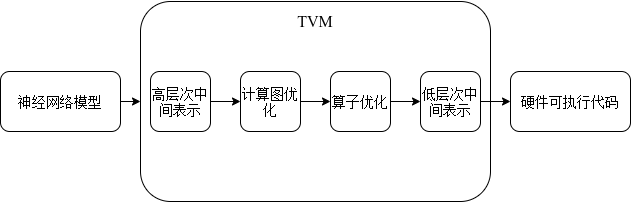
\includegraphics[width=270bp]{figure/tvm_overview.png}
    \caption{TVM编译流程}
    \label{tvm_overivew}
\end{figure}

如图\ref{tvm_overivew}所示,TVM的具体执行流程为,对于不同深度学习框架训练得到的模型转化为统一的高层次中间表示,然后对该中间表示进行一些计算图层面的优化,如数据流重写等,得到一个优化的计算图。之后把高层次的中间表示转化为低层次的中间表示,并进行算子层面的优化,如算子的合并,同时针对不同不同硬件设备的内存和指令结构进行具体的优化。

\section{研究内容}

本论文基于TVM,通过具体实践TVM的编译部署流程,来对TVM的编译部署流程进行封装,同时设计并实现一个简洁,统一的接口,来让用户进行调用。总的来说,本论文的研究内容有这样几个方面,平台环境配置,工具链构建,TVM模型编译部署流程,平台的设计与实现,平台测试。

\subsection{环境配置}

为了实现多框架和多设备的支持,平台后端需要复杂的环境。如表\ref{base_environment}所示,平台需要工具构建的一些编译软件,GPU的一些计算库,各个深度学习框架的Python库,构建安卓应用时所依赖的安卓开发工具(Android SDK,Android Software Development Kit),JAVA开发工具(JDK,Java Development Kit),和GPU的驱动等等。平台实现了上述软件的安装,以及解决了软件之间的版本依赖问题。

\begin{table}
    \centering
    \caption{平台环境}
    \label{base_environment}
    \begin{tabular}{c||c}
        \hline
        驱动         & Nidia Driver \\ \hline
        GPU计算库    & Cuda, Cudnn, OpenCL \\ \hline
        深度学习框架  & Pytorch, Tensorflow, Keras, Onnx, MXNet \\ \hline
        Android SDK & Emulator, Build Tools, Ndk, Platform Tools, Cmdline Tools \\ \hline
        构建工具     & GCC, LLVM, CMake, Make, Maven, Gradle \\ \hline
        JAVA        & JDK \\ \hline
    \end{tabular}
\end{table}


\subsection{工具链构建}

本研究所依赖的部分工具没有构建好的软件包,还需要从源码进行构建。

首先,需要构建本平台依赖的TVM工具,使用CMake和Make工具来编译TVM的动态连接库(libtvm.so),为了使平台能够支持多种设备和计算平台,还需要依赖Cuda,Cudnn,OpenCL,LLVM等动态连接库。编译好TVM的动态连接库后需要打包为Python的库,使得能够通过TVM的Python前端来使用TVM。

其次,该平台需要把神经网络模型部署到安卓设备上,所以还需要构建TVM的Java前端。使得用户能够使用Java来调用部署到安卓设备上的模型。

最后,因为该平台需要把模型部署在安卓设备上,所以需要一个安卓软件来使安卓设备和本地电脑进行通信。在构建安卓软件时需要依赖Android SDK等软件,使用Maven和Gradle进行软件的构建。

\subsection{模型编译与部署}

该平台支持了多种深度学习框架,通过调用对应框架的API实现了每种框架模型的加载和保存。并且该平台通过调用TVM的API实现了不同框架模型的编译,能够得到统一的中间计算图表示和模型参数。同时该平台实现了服务器端CPU的部署,以及服务器端GPU上Cuda和OpenCL等计算平台的部署,实现了安卓设备的CPU的部署和GPU上OpenCL和Vulkan等计算平台的部署,同时实现了树莓派和FPGA端的部署。

\subsection{接口设计}

该平台设计并实现了一个简洁通一的接口。用户通过调用该接口来实现模型到硬件设备的端到端的部署。接口通过几个关键的变量来实现多框架和多设备的支持。Frame(框架)表示用户输入模型的框架种类。Device(设备)表示用户希望部署到的硬件设备。Target(目标计算平台)表示用户希望部署到的计算平台,该变量与具体的部署的硬件设备相关。通过这个接口,用户能够得到部署好的模型\verb|deploy_model|。与主流的深度学习框架的使用方式相同,用户能够通过\verb|deploy_model(input)|来获得模型的输出。

\subsection{平台测试}

该平台实现充分的测试,对平台对所支持框架和硬件设备进行了充分的测试。


